\documentclass[%
	11pt,
	a4paper,
	utf8,
	%twocolumn
		]{article}	

\usepackage{style_packages/podvoyskiy_article_extended}


\begin{document}
\title{Заметки по машинному обучению и анализу данных. Том 2}

\author{\itshape Подвойский А.О.}

\date{}
\maketitle

\thispagestyle{fancy}

Здесь приводятся заметки по некоторым вопросам, касающимся машинного обучения, анализа данных, программирования на языках \texttt{Python}, \texttt{R} и прочим сопряженным вопросам так или иначе, затрагивающим работу с данными.


\shorttableofcontents{Краткое содержание}{1}

\tableofcontents

\section{Приемы работы с библиотеками Gym и Ecole}

\subsection{Gym}

Функция окружения (environment) \texttt{step} возвращает четыре значения:
\begin{itemize}
	\item \verb|observation| (object):  это объект, специфичный для окружающей среды и представляющий результат наблюдения за этой средой (например, состояние доски в настольной игре),
	
	\item \verb|reward| (float): вознаграждение, полученное за предыдущее действие. Масштаб варьируется в зависимости от среды, но цель всегда в том, чтобы сделать суммарное вознаграждение как можно больше,
	
	\item \verb|done| (boolean): флаг завершения эпизода. Многие (но не все) задачи разделены на четко определенные эпизоды, и \texttt{done = True} указывает на то, что эпизод завершился (например, мы потеряли последнюю жизнь в игре),
	
	\item \verb|info| (dict): диагонстическая информация, полезная для отладки.
\end{itemize}

Это просто реализация классического цикла <<агент -- среда>>. На каждом шаге агент совершает то или иное действие и среда возвращает наблюдения (observation) и вознаграждение (reward).

Процесс запускается вызовом функции \verb|reset()|, которая возвращает первое приближение \texttt{observation}.  
\begin{lstlisting}[
style=ironpython,
numbers=none
]
import gym
env = gym.make('CartPole-v0')
for i_episode in range(20):
    observation = env.reset()
    for t in range(100):
        env.render()
        print(observation)
        action = env.action_space.sample()
        observation, reward, done, info = env.step(action)
        if done:
            print("Episode finished after {} timesteps".format(t+1))
            break
env.close()
\end{lstlisting}

В этом примере мы отбирали случайные действия из пространства действий среды. Каждая среда поставляется с атрибутами \verb|action_space| и \verb|observation_space|. Эти атрибуты имеют тип \verb|Space| и описывают формат допустимых действий и наблюдений
\begin{lstlisting}[
style=ironpython,
numbers=none
]
import gym

env = gym.make("CartPole-v0")
print(env.action_space)  # Discrete(2)

print(env.observation_space)  # Box([-4.8000002e+00 -3.4028235e+38 -4.1887903e-01 -3.4028235e+38], [4.8000002e+00 3.4028235e+38 4.1887903e-01 3.4028235e+38], (4,), float32)
\end{lstlisting}

Пространство \texttt{Descrete} описывает фиксированный диапазон неотрицательных чисел, так что в данном случае допустимыми действиями будет 0 или 1. Пространство \texttt{Box} представляет $ n $-мерный ящик, так что в данном случае допустимыми наблюдениями будут 4-мерные массивы.

\subsection{Ecole}

Полезный ресурс о специальных приемах работы с задачами линейного программирования в частично-целочисленного постановке \url{https://www.gams.com/37/docs/UG_LanguageFeatures.html?search=sos1}

Полезный ресурс по математической оптимизации \url{https://scipbook.readthedocs.io/en/latest/}

\subsubsection{Observations}

Класс \texttt{ecole.observation.NodeBipartiteObs}: двудольный граф наблюдений для узлов branch-and-bound дерева. Оптимизационная задача представляется в виде гетерогенного двудольного графа. Между переменной и ограничением будет существовать ребро, если переменная присутствует в ограничении с ненулевым коэффициентом.

Метод \texttt{reset()} в Ecole принимает в качестве аргумента экземпляр проблемы. 

\section{Отбор признаков с библиотекой BoostARoota}

BoostARoota \url{https://github.com/chasedehan/BoostARoota} -- алгоритм отобора признаков на базе экстримального градиентного бустинга в реализации XGBoost. Алгоритм требует гораздо меньших затрат времени на выполнение. Перед применением необходимо выполнить дамми-кодирование, поскольку базовая модель работает только с количественными признаками.

Отбор признаков выполняется на обучающем поднаборе данных, поэтому предполагается, что массив меток и массив признаков \emph{обучающие}, а для проверки качества модели отбора признаков есть независимая, \emph{тестовая} выборка. Кроме того, если необходимо выбрать оптимальные значения гиперпараметров модели отбора признаков (например, значения гиперпараметров \texttt{cutoff}, \texttt{iters} и \texttt{delta}), то понадобиться еще \emph{проверочная} {выборка}.

\section{Площадь по ROC-кривой}

Построение ROC-кривой происходит следующим образом (\pic{fig:roc_auc0}):
\begin{enumerate}
	\item  Сначала сортируем все наблюдения по убыванию спрогнозированной вероятности положительного класса,
	
	\item Берем единичный квадрат на координатной плоскости. Значения оси абсцисс будут значениями 1 - специфичности (цена деления оси задается значением 1/neg), а значения оси ординат будут значениями чувствительности (цена деления оси задается значением 1/pos). При этом pos — это количество наблюдений положительного класса, а neg — количество наблюдений отрицательного класса,
	
	\item Задаем точку c координатами (0, 0) и для каждого отсортированного наблюдения x:
	\begin{itemize}
		\item если x принадлежит положительному классу, двигаемся на 1/pos вверх,
		
		\item если x принадлежит отрицательному классу, двигаемся на 1/neg вправо.
	\end{itemize}
\end{enumerate}

Значение вероятности положительного класса, при котором ROC-кривая находится на минимальном расстоянии от верхнего левого угла -- точки с координатами (0, 1), дает наибольшую правильность классификации. В данному случае (\pic{fig:roc_auc0-1}) будет 0.72.

\begin{figure}[h]
	\centering
	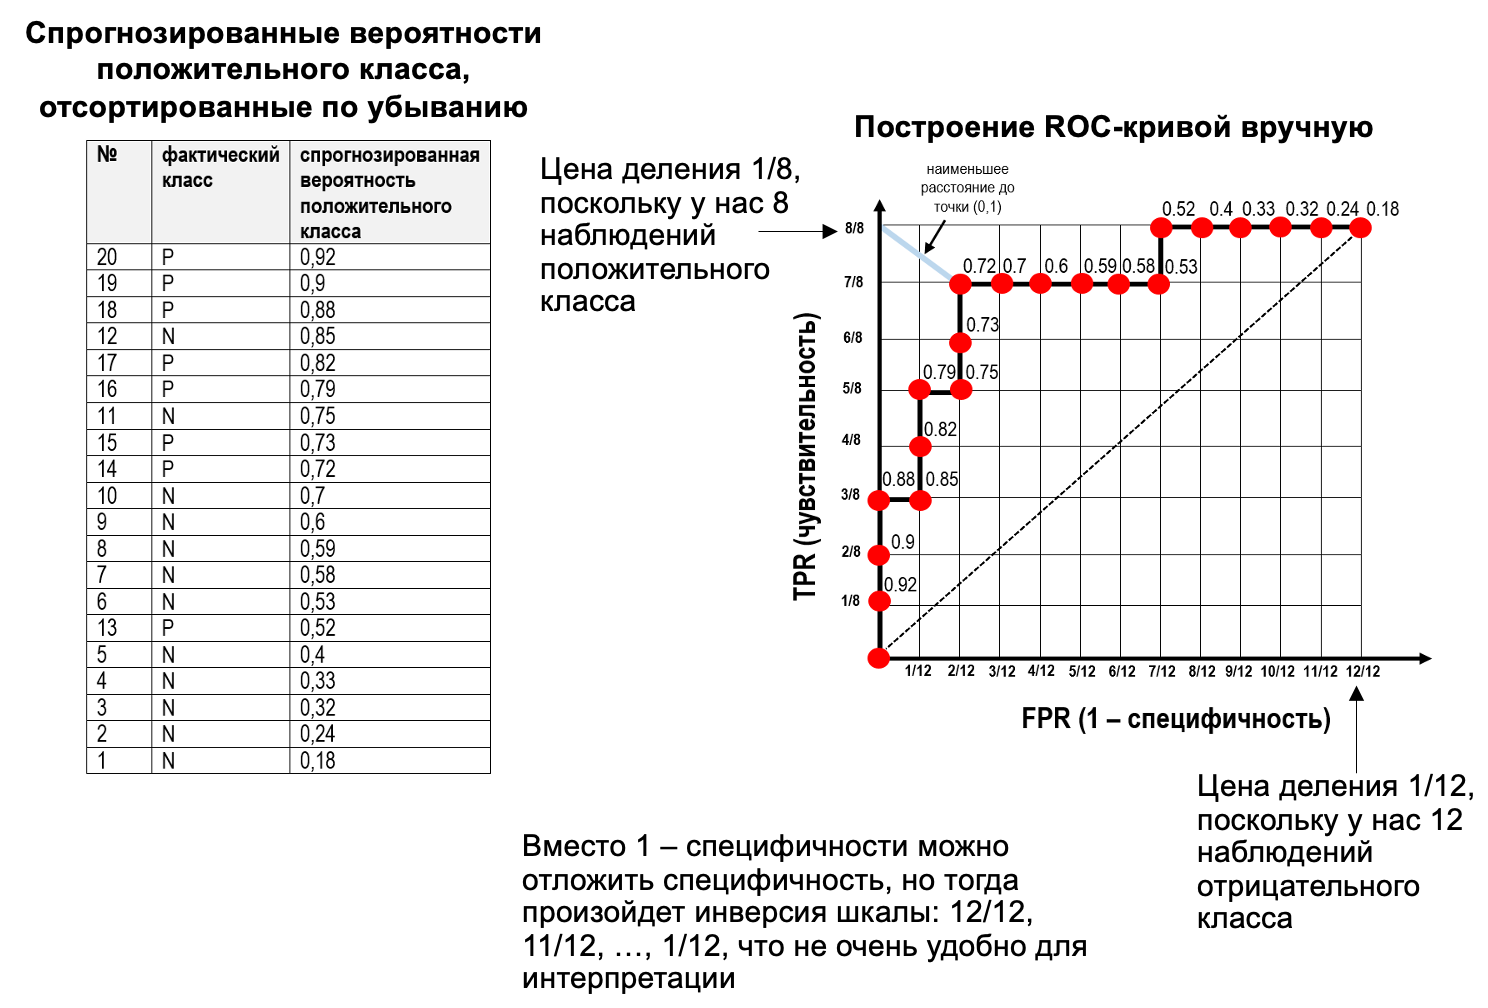
\includegraphics[scale=0.3]{figures/roc_auc0.png}
	\caption{ Построение ROC-кривой }\label{fig:roc_auc0}
\end{figure}

\begin{figure}[h]
	\centering
	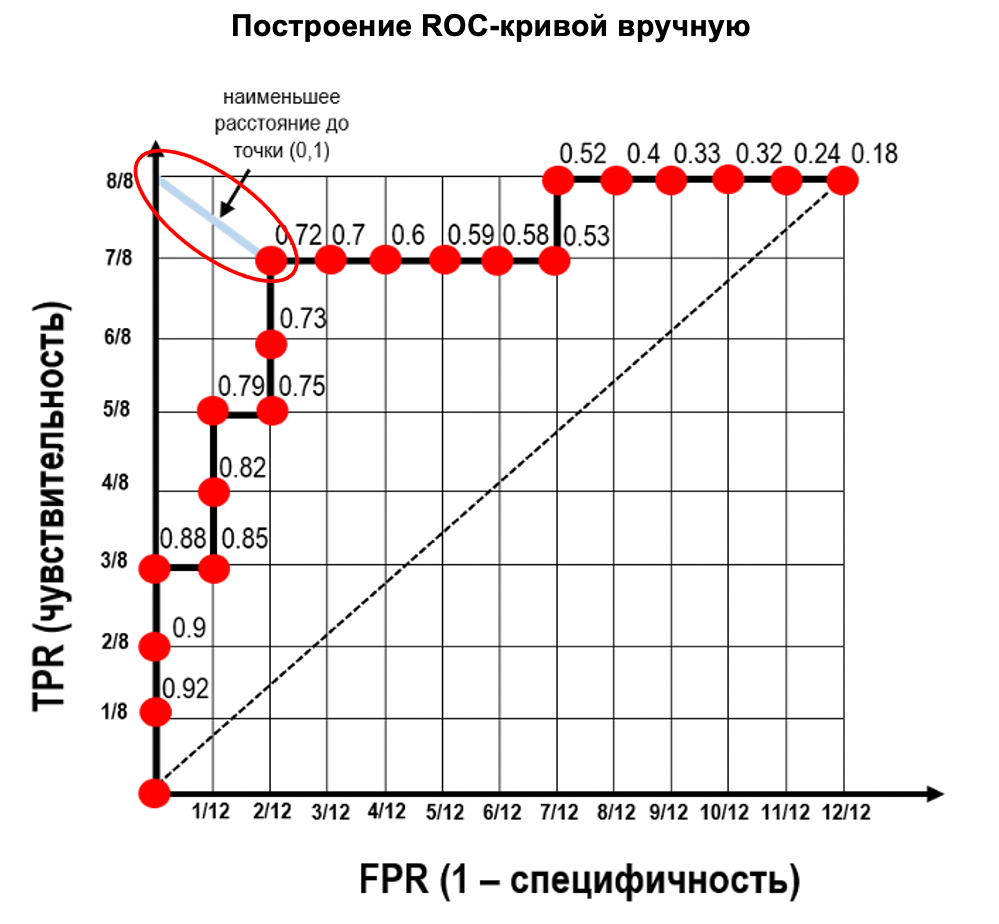
\includegraphics[scale=0.3]{figures/roc_auc0-1.png}
	\caption{ ROC-кривая. Порог отсечения 0.72 }\label{fig:roc_auc0-1}
\end{figure}

Площадь под ROC-кривой (ROC-AUC) можно интерпретировать как вероятность события, состоящего в том, что классификатор присвоит более высокий ранг (например, вероятность) случайно выбранному экземпляру положительного класса, чем случайно выбранному экземпляру отрицательного класса (если не рассматривать вариант равенства значений рангов).

\remark{
На ROC-кривые не влияет баланс классов (при достаточном объеме выборки) и они могут чрезмерно оптимистично оценивать качество работы алгоритма в случае дисбалансов. Лучше пользоваться гармоническим средним или PR-кривыми
}

Однако недостаток такой интепретации заключается в том, что мы пренебрегаем часто встречающейся ситуацией равенства вероятностей. Поэтому правильнее будет сказать, что ROC-AUC равен доле пар вида (экземпляр положительного класса, экземпляр отрицательного класса), которые алгоритм верно упорядочил в соответствии с формулой
\begin{align}\label{eq:rocauc}
	\dfrac{ \sum\limits_{i, j=1}^{n_i, n_j} s(x_i, x_j)}{ n_i \, n_j }, \quad s(x_i, x_j) =
	\begin{cases}
		1, x_i > x_j,\\
		1/2, x_i = x_j,\\
		0, x_i < x_j,
	\end{cases}
\end{align}
где $ x_i $ -- ответ алгоритма для положительного экземпляра, $ x_j $ -- ответ алгоритма для отрицательного экземпляра.

По сути числитель дроби представляет собой сумму количеств $ j $-ых наблюдений отрицательного класса, лежащих ниже каждого $ i $-ого наблюдения положительного класса. Каждое такое количество мы берем по каждому $ i $-ому наблюдению положительного класса в последовательности, отсортированной по мере убывания вероятности положительного класса. Знаменатель дроби -- это произведение количества наблюдений положительного класса и наблюдений отрицательного класса.

Если говорить более точно, мы берем наблюдение положительного класса под номером 20 и каждый раз образовываем пару с наблюдением отрицательного класса (\ref{fig:roc_auc1}), у нас 12 пар, 12 раз наблюдение полжительного класса под номером 20 было проранжировано выше наблюдений отрицательного класса 12, 11, 10 и т.д. Записываем число 12 напротив наблюдения 20. 

Разные модели нельзя сравнивать только по ROC-AUC. ROC-AUC оценивает разные классификатор, используя метрику, которая сама зависит от классификатора. То есть ROC-AUC оценивает разные классификаторы, используя разные метрики.

\remark{
Если часть ROC-кривой лежит ниже диагональной линии, а часть -- выше, то это означает, что классы не являются линейно-сепарабельными, а при этом используется линейная модель
}

При одинаковой ROC-AUC у разных моделей (соответственно с разными ROC-кривыми) будет разное распределение стоимостей ошибочной классификации. Проще говоря, мы можем вычислить ROC-AUC для классификатора A и получить 0.7, а затем вычислить ROC-AUC для второго классификатора и снова получить 0.7, но это не обязательно означает, что у них одна и та же эффективность.

\begin{figure}[h]
	\centering
	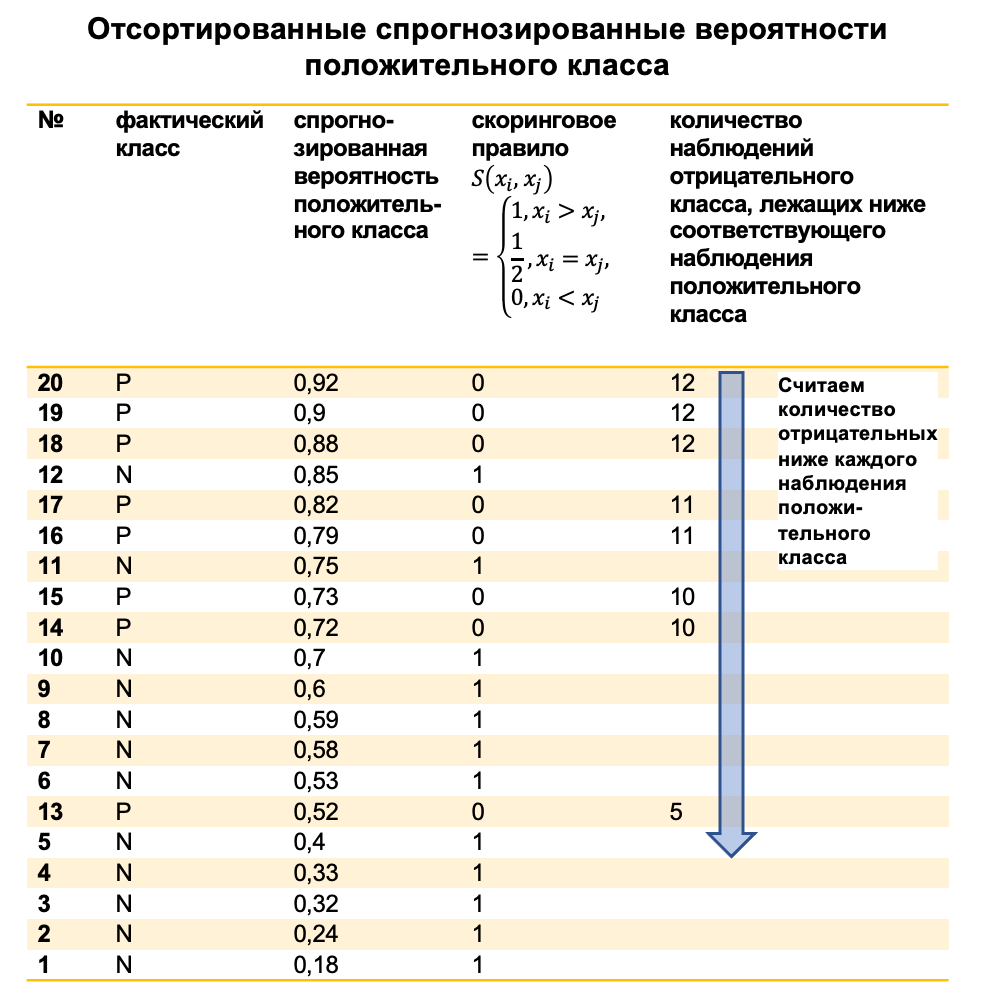
\includegraphics[scale=0.35]{figures/roc_auc1.png}
	\caption{ Расчет ROC-AUC по формуле \eqref{eq:rocauc}}\label{fig:roc_auc1}
\end{figure}

\begin{figure}[h]
	\centering
	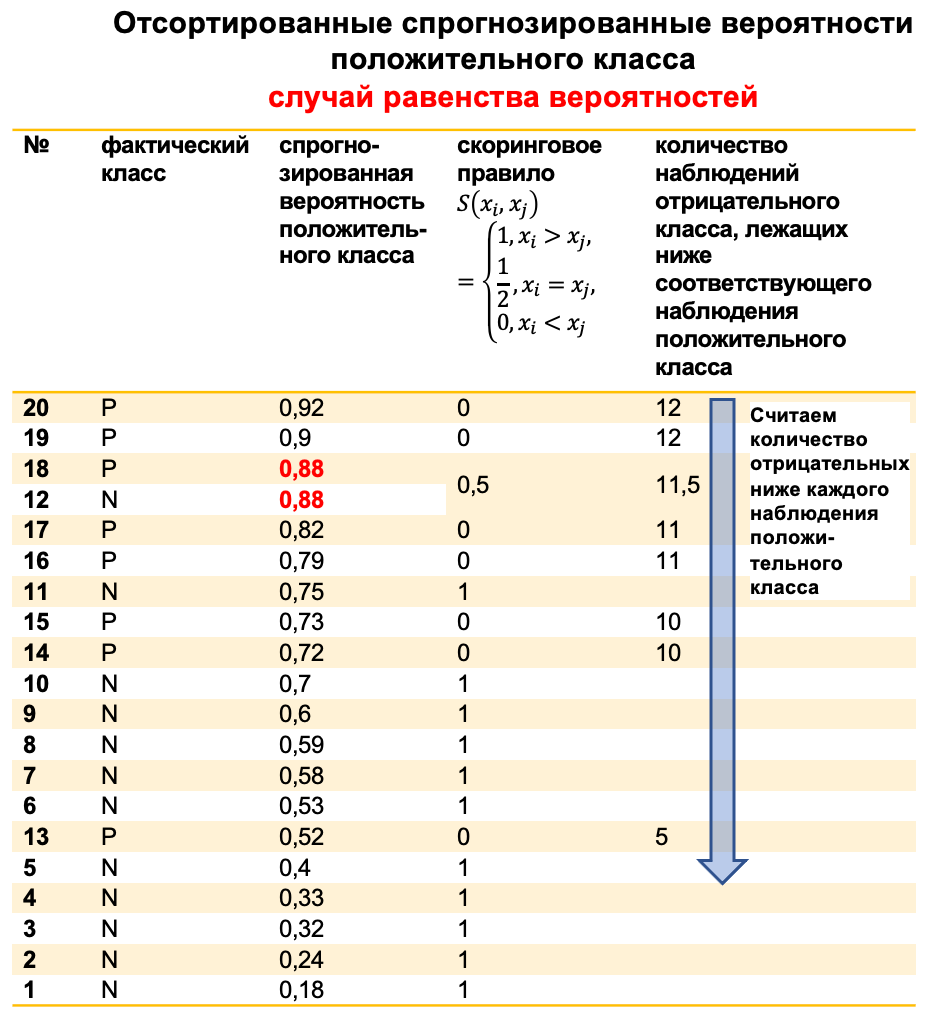
\includegraphics[scale=0.35]{figures/roc_auc2.png}
	\caption{ Расчет ROC-AUC по формуле \eqref{eq:rocauc} для случая равных вероятностей принадлежности экземпляра положительному классу}\label{fig:roc_auc2}
\end{figure}




\listoffigures\addcontentsline{toc}{section}{Список иллюстраций}

% Источники в "Газовой промышленности" нумеруются по мере упоминания 
\begin{thebibliography}{99}\addcontentsline{toc}{section}{Список литературы}
	\bibitem{lutz:learningpython-2011}{\emph{Лутц М.} Изучаем Python, 4-е издание. -- Пер. с англ. -- СПб.: Символ-Плюс, 2011. -- 1280~с. }
		
	\bibitem{beazley:python-2010}{\emph{Бизли Д.} Python. Подробный справочник. -- Пер. с англ. -- СПб.: Символ-Плюс, 2010. -- 864~с. }
\end{thebibliography}

\end{document}
